% Options for packages loaded elsewhere
\PassOptionsToPackage{unicode}{hyperref}
\PassOptionsToPackage{hyphens}{url}
\PassOptionsToPackage{dvipsnames,svgnames,x11names}{xcolor}
%
\documentclass[
  letterpaper,
  DIV=11,
  numbers=noendperiod]{scrartcl}

\usepackage{amsmath,amssymb}
\usepackage{lmodern}
\usepackage{iftex}
\ifPDFTeX
  \usepackage[T1]{fontenc}
  \usepackage[utf8]{inputenc}
  \usepackage{textcomp} % provide euro and other symbols
\else % if luatex or xetex
  \usepackage{unicode-math}
  \defaultfontfeatures{Scale=MatchLowercase}
  \defaultfontfeatures[\rmfamily]{Ligatures=TeX,Scale=1}
\fi
% Use upquote if available, for straight quotes in verbatim environments
\IfFileExists{upquote.sty}{\usepackage{upquote}}{}
\IfFileExists{microtype.sty}{% use microtype if available
  \usepackage[]{microtype}
  \UseMicrotypeSet[protrusion]{basicmath} % disable protrusion for tt fonts
}{}
\makeatletter
\@ifundefined{KOMAClassName}{% if non-KOMA class
  \IfFileExists{parskip.sty}{%
    \usepackage{parskip}
  }{% else
    \setlength{\parindent}{0pt}
    \setlength{\parskip}{6pt plus 2pt minus 1pt}}
}{% if KOMA class
  \KOMAoptions{parskip=half}}
\makeatother
\usepackage{xcolor}
\setlength{\emergencystretch}{3em} % prevent overfull lines
\setcounter{secnumdepth}{-\maxdimen} % remove section numbering
% Make \paragraph and \subparagraph free-standing
\ifx\paragraph\undefined\else
  \let\oldparagraph\paragraph
  \renewcommand{\paragraph}[1]{\oldparagraph{#1}\mbox{}}
\fi
\ifx\subparagraph\undefined\else
  \let\oldsubparagraph\subparagraph
  \renewcommand{\subparagraph}[1]{\oldsubparagraph{#1}\mbox{}}
\fi


\providecommand{\tightlist}{%
  \setlength{\itemsep}{0pt}\setlength{\parskip}{0pt}}\usepackage{longtable,booktabs,array}
\usepackage{calc} % for calculating minipage widths
% Correct order of tables after \paragraph or \subparagraph
\usepackage{etoolbox}
\makeatletter
\patchcmd\longtable{\par}{\if@noskipsec\mbox{}\fi\par}{}{}
\makeatother
% Allow footnotes in longtable head/foot
\IfFileExists{footnotehyper.sty}{\usepackage{footnotehyper}}{\usepackage{footnote}}
\makesavenoteenv{longtable}
\usepackage{graphicx}
\makeatletter
\def\maxwidth{\ifdim\Gin@nat@width>\linewidth\linewidth\else\Gin@nat@width\fi}
\def\maxheight{\ifdim\Gin@nat@height>\textheight\textheight\else\Gin@nat@height\fi}
\makeatother
% Scale images if necessary, so that they will not overflow the page
% margins by default, and it is still possible to overwrite the defaults
% using explicit options in \includegraphics[width, height, ...]{}
\setkeys{Gin}{width=\maxwidth,height=\maxheight,keepaspectratio}
% Set default figure placement to htbp
\makeatletter
\def\fps@figure{htbp}
\makeatother

\KOMAoption{captions}{tableheading}
\makeatletter
\makeatother
\makeatletter
\makeatother
\makeatletter
\@ifpackageloaded{caption}{}{\usepackage{caption}}
\AtBeginDocument{%
\ifdefined\contentsname
  \renewcommand*\contentsname{Table of contents}
\else
  \newcommand\contentsname{Table of contents}
\fi
\ifdefined\listfigurename
  \renewcommand*\listfigurename{List of Figures}
\else
  \newcommand\listfigurename{List of Figures}
\fi
\ifdefined\listtablename
  \renewcommand*\listtablename{List of Tables}
\else
  \newcommand\listtablename{List of Tables}
\fi
\ifdefined\figurename
  \renewcommand*\figurename{Figure}
\else
  \newcommand\figurename{Figure}
\fi
\ifdefined\tablename
  \renewcommand*\tablename{Table}
\else
  \newcommand\tablename{Table}
\fi
}
\@ifpackageloaded{float}{}{\usepackage{float}}
\floatstyle{ruled}
\@ifundefined{c@chapter}{\newfloat{codelisting}{h}{lop}}{\newfloat{codelisting}{h}{lop}[chapter]}
\floatname{codelisting}{Listing}
\newcommand*\listoflistings{\listof{codelisting}{List of Listings}}
\makeatother
\makeatletter
\@ifpackageloaded{caption}{}{\usepackage{caption}}
\@ifpackageloaded{subcaption}{}{\usepackage{subcaption}}
\makeatother
\makeatletter
\@ifpackageloaded{tcolorbox}{}{\usepackage[many]{tcolorbox}}
\makeatother
\makeatletter
\@ifundefined{shadecolor}{\definecolor{shadecolor}{rgb}{.97, .97, .97}}
\makeatother
\makeatletter
\makeatother
\ifLuaTeX
  \usepackage{selnolig}  % disable illegal ligatures
\fi
\IfFileExists{bookmark.sty}{\usepackage{bookmark}}{\usepackage{hyperref}}
\IfFileExists{xurl.sty}{\usepackage{xurl}}{} % add URL line breaks if available
\urlstyle{same} % disable monospaced font for URLs
\hypersetup{
  pdftitle={The expected utilization of postage batches},
  pdfauthor={The Swarm Authors},
  colorlinks=true,
  linkcolor={blue},
  filecolor={Maroon},
  citecolor={Blue},
  urlcolor={Blue},
  pdfcreator={LaTeX via pandoc}}

\title{The expected utilization of postage batches}
\author{The Swarm Authors}
\date{}

\begin{document}
\maketitle
\ifdefined\Shaded\renewenvironment{Shaded}{\begin{tcolorbox}[boxrule=0pt, sharp corners, frame hidden, interior hidden, borderline west={3pt}{0pt}{shadecolor}, breakable, enhanced]}{\end{tcolorbox}}\fi

When pushing content to the Swarm network, uploaders are required to
attach an attestation of storage rent prepayment to each chunk they
post. The latter is essentially a wallet registered on the postage
contract seeded with a balance from which storage rent is deduced by the
network-wide incentive system. Since this is reminiscent of buying a
batch of postage stamps and attaching one to each envelope to be posted,
the attestations are called \emph{postage stamps} and the registered
wallet a \emph{postage batch.} One can think of batches as collections
of \emph{storage slots.} The size of a batch is the number of storage
slots and is always specified as $2^d$, where the exponent $d$ is
called the \emph{batch depth.} Each slot can hold at most one chunk.
Putting a chunk into a slot is like issuing a postage stamp.

In practice, the attached postage stamps are digital signatures which
associate the address of a chunk with a \emph{storage slot reference.}
This in turn is composed of 1) a reference to the wallet through its
\emph{batch ID,} and 2) a \emph{within-batch index.} The fact that each
slot can hold at most one chunk ensures that batches cannot issue more
stamps than the volume registered with them. However, for an
\emph{overissuance} incident to be detectable locally by storer nodes,
the within-batch indices are arranged such that the highest $n$ bits
match the prefix of the chunk they are assigned to, and therefore will
all be stored within the locality of the network. These $n$ bits
define $2^n$ \emph{buckets,} within the buckets, the index is
sequentially assigned to chunks and therefore allows collisions. The log
number of buckets $n$ is thus called the \emph{collision depth.} If
the overall batch size is characterized by batch depth $d$ and there
are $2^n$ buckets, then each bucket will hold a maximum of $2^{d-n}$
chunks. $k=d-n$ is the log size of a bucket ($2^k$ is the
\emph{bucket depth}), and it provides an exclusive upper bound to
within-bucket indices.

Overusing a batch is now easily detected by any storer node as long as
their storage depth is not larger than the batch's collision depth. In
that case, each bucket of a batch is entirely within the node's reserve.
Overissuance is therefore immediately caught, since the multiple chunks
assigned to the same slot index are seen by any node in that
neighbourhood.

When all slots are filled, we say the batch is \emph{fully utilized.}
Although the \emph{a priori} distribution of chunks is uniform (and
therefore the expected number of chunks falling into each bucket is the
same), their stochastic assignment means that it is practically
impossible to fill all buckets without eventually attempting to add to
one that is already full. We assume that the uploader is unable to
affect the address of the chunk (unencrypted fixed content) that falls
into such already-filled buckets, and therefore they are unable to
continue uploading. Because of this, one may legitimately consider the
batch to be no longer usable. The number of stamps hitherto issued by
the batch is called its \emph{effective batch size,} and its ratio to
the batch size its \emph{batch utilization rate.}

Below we explore the effect of batch parameters on their utilization
rate. With an insight into utilization rates as a function of the number
of buckets $2^n$ and the size of buckets $2^k$, we will have a way
to calibrate the expected effective batch size to be presented to users
in the context of a batch purchase user experience.

The problem of assigning chunks to storage slots is analogous with the
process of throwing marbles, one after the other, in boxes which are
initially empty. Each throw may end up in any of the boxes with equal
probability, and thus the marbles get distributed across the boxes more
or less evenly through time. However, the time will come when the boxes
start filling up. At that point, a marble may by chance end up being
thrown into a box that is already full, and thus get rejected.
Substituting chunks for marbles, buckets for boxes, and the act of
signing a stamp for throwing a marble, we recover our original scenario.
Marbles ending up in a box with equal probability corresponds to the
fact that a random chunk has equal chance of being assigned to a bucket
since the hash function has uniform distribution. Repeated rounds of
marble throwing correspond to consecutive stamping of multiple chunks of
the uploaded content; rounds constitute repeated independent trials.

Taking a particular bucket, each round of stamping is a ``success'' if
the stamp falls into the bucket, and a ``failure'' otherwise. Due to the
fact that a marble may end up in each box with equal chance, the
probability of success is $1/n$ and the probability of failure is
$1 - 1/n$. The number of stamps issued to the bucket after a given
number of rounds is described by the
\href{https://en.wikipedia.org/wiki/Negative_binomial_distribution\#Distribution_of_a_sum_of_geometrically_distributed_random_variables}{negative
binomial distribution} $\mathcal{B}(k, 1/n)$, where the first
parameter $k$ is the number of failed rounds before we stop counting,
and the second parameter is the probability of success.

The negative binomial distribution $\mathcal{B}(k, 1/n)$ is equivalent
to the sum of $k$ independent geometrically distributed variables with
parameter $1/n$. Unless $k$ is very small, the central limit theorem
ensures that this sum converges to a normal distribution. Formally, if
$\mathcal{Y}_i(1/n)$ are independent geometrically distributed
variables with parameter $1/n$, and $\mathcal{N}(\mu, \sigma^2)$ is
the normal distribution with mean $\mu$ and variance $\sigma^2$,
then for large $k$ we have
\begin{equation}\protect\hypertarget{eq-binomial-approximation}{}{
\mathcal{B}(k, 1/n) = \sum_{i=1}^k \mathcal{Y}_i(1/n) \approx \mathcal{N}(kn, kn(n-1))
}\label{eq-binomial-approximation}\end{equation} The reason for the
above form of the mean and variance in the normal distribution is as
follows: given a single geometrically distributed variable with
parameter $1/n$, its mean is $n$ and its variance is $n(n-1)$.
When adding these up over $k$ independent variables, we arrive at
$\mu = k n$ and $\sigma^2 = k n (n - 1)$ in the limiting normal
distribution.

The fit of the normal distribution with the binomial is robust even for
low values of $k$, as depicted in Figure~\ref{fig-normal-binomial}.

\begin{figure}

{\centering 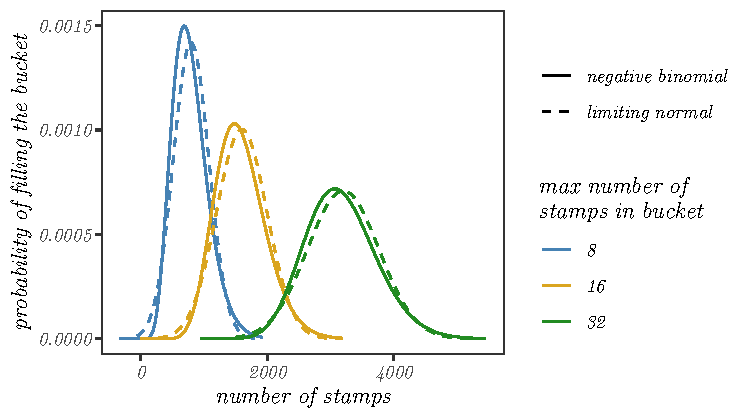
\includegraphics[width=0.7\textwidth,height=\textheight]{postage_batch_utilization_figs/fig-normal-binomial-1.pdf}

}

\caption{\label{fig-normal-binomial}Approximating negative binomial
distributions with limiting normal ones. The number of buckets \emph{n}
is fixed at 100.}

\end{figure}

The negative binomial distribution estimates the number of rounds a
particular bucket fills up, given its size $k$ and the number of
buckets $n$. The rounds of stamping can be conceived of as parallel
independent attempts at filling up buckets. Stamps issued for failed
rounds still end up in one of the other $n - 1$ buckets, and therefore
the same probability variable counts the total stamps issued by the
batch in all buckets at the time the first one fills up. Thus, we want
to know how the \emph{minimum} of $n$ independent normal variates,
$X = \min_{i \in \{1\ldots n\}} \mathcal{N}_i(\mu, \sigma^2)$, is
distributed.

This so-called \emph{extreme value distribution} would give us the
distribution of the absolute number of total rounds needed until the
first event when one of the buckets fills up. Therefore its mean is
exactly the expected value of the number of rounds until the first
bucket-filling event. Since this is when the batch is considered
effectively used up, the mean of the distribution measures the effective
utilization of the batch. Dividing by $n$ gives the expected number of
stamps per bucket making the rate comparable across any parameter of
bucket size. Further dividing by $k$ in turn gives the \emph{expected
normalized utilization rate}, which is now comparable across all $k$
and $n$ values.

The extreme value distribution for the minimum of $n$ independent
variates drawn from the standard normal distribution (with zero mean and
unit variance) is known. It is the
\href{https://en.wikipedia.org/wiki/Gumbel_distribution}{Gumbel
distribution}, which reads
\begin{equation}\protect\hypertarget{eq-gumbel}{}{
\mathcal{G}(x; \alpha, \beta) = \frac{1}{\beta} \exp\left[
\frac{x + \alpha}{\beta} - \exp\left(\frac{x + \alpha}{\beta}\right)\right] .
}\label{eq-gumbel}\end{equation} Here $x$ is the independent variable
(in our case, the number of rounds of stamping), and $\alpha$ and
$\beta$ are the \emph{location} and \emph{scale} parameters,
respectively.\footnote{The Gumbel distribution is often given using the
  convention that one is looking for the maximum of $n$ normal
  variates, instead of their minimum. One can change between the two by
  simply flipping the sign of $x$.} They are in turn given by
\begin{equation}\protect\hypertarget{eq-loc-scale}{}{
\begin{aligned}
  \alpha &= \rho\left( 1 - \frac{1}{n} \right) ,
  \\
  \beta &= \rho\left( 1 - \frac{\text{e}^{-1}}{n} \right) - \alpha ,
\end{aligned}
}\label{eq-loc-scale}\end{equation} where
$\text{e}^{-1} = \exp(-1) \approx 0.368$, $n$ is the number of
normal variates whose minimum we are looking for, and $\rho(x)$ is the
quantile function of the normal distribution (or the inverse of the
\href{https://en.wikipedia.org/wiki/Error_function}{error function}).
The mean, standard deviation, and quantile function of the Gumbel
distribution are
\begin{equation}\protect\hypertarget{eq-mean-var-quantile}{}{
\begin{aligned}
  \mathbb{E}(\mathcal{G}) &= \alpha + \gamma \beta ,
  \\
  \mathbb{S}(\mathcal{G}) &= \beta \, \frac{\pi}{\sqrt{6}} ,
  \\
  Q(p; \mathcal{G}) &= \beta \, \log(-\log(1 - p)) - \alpha ,
\end{aligned}
}\label{eq-mean-var-quantile}\end{equation} where
$\gamma \approx 0.5772$ is the Euler--Mascheroni constant, and
$0 < p < 1$ in $Q(p; \mathcal{G})$ is a probability quantile.

The normal distribution whose variates' minimum values we are looking
for is not standard, but instead has mean $\mu = k n$ (instead of
zero), and variance $\sigma^2 = k n (n-1)$ (instead of one).
Therefore, the Gumbel distribution needs to be appropriately rescaled.
Denoting this scaled probability distribution by $\mathcal{X}$, we
have \begin{equation}\protect\hypertarget{eq-gumbel-scaled}{}{
  \mathcal{X}(x; \mu, \sigma, \alpha, \beta) =
  \frac{1}{\sigma}\mathcal{G}\left(\frac{x - \mu}{\sigma}; \alpha, \beta\right)
}\label{eq-gumbel-scaled}\end{equation} (the overall factor of
$1 / \sigma$ restores the proper normalization of the scaled
function). Consequently, the mean, standard deviation, and quantile
function should also be rescaled:
\begin{equation}\protect\hypertarget{eq-mean-var-quantile-scaled}{}{
\begin{aligned}
  \mathbb{E}(\mathcal{X}) &= \mu - \sigma (\alpha+\gamma\beta) = kn-\sqrt{kn(n-1)}
  \left[(1-\gamma) \rho\left( 1 - \frac{1}{n} \right) + \gamma \rho\left( 1 -
  \frac{\text{e}^{-1}}{n} \right) \right] , 
  \\
  \mathbb{S}(\mathcal{X}) &=\sigma \beta \frac{\pi}{\sqrt{6}} =
  \sqrt{ k n (n-1)} \left[ \rho\left( 1 - \frac{\text{e}^{-1}}{n} \right) -
  \rho\left( 1 - \frac{1}{n} \right) \right] \frac{\pi}{\sqrt{6}} ,
  \\
  Q(p;\mathcal{X})&= \mu-\sigma\left[\alpha-\beta \,
  \log(-\log(1-p))\right] \\ &= kn-\sqrt{ k n (n-1)}\left[\rho\left( 1 -
  \frac{1}{n} \right)-\rho\left( 1 - \frac{\text{e}^{-1}}{n} \right) 
  \log\left(-\log(1-p)\right)\right] .
\end{aligned}
}\label{eq-mean-var-quantile-scaled}\end{equation} Normalizing the mean
and the quantile function by the product $kn$:
\begin{equation}\protect\hypertarget{eq-mean-quant-div}{}{
\begin{aligned}
  \frac{\mathbb{E}(\mathcal{X})}{k n} &= 1 - \sqrt{\frac{(n-1)}{kn}} \left[ (1-\gamma)
  \rho\left( 1 - \frac{1}{n} \right) + \gamma \rho\left( 1 - \frac{\text{e}^{-1}}{n}
  \right) \right] ,
  \\
  \frac{Q(p; \mathcal{X})}{kn} &= 1 - \sqrt{\frac{(n-1)}{kn}}
  \left[\rho\left( 1 - \frac{1}{n} \right)-\rho\left( 1 - \frac{\text{e}^{-1}}{n}
  \right)  \log\left(-\log(1-p)\right)\right] .
\end{aligned}
}\label{eq-mean-quant-div}\end{equation} Taking into account that $k$
and $n$ must both be powers of two, we can write $k = 2^{\kappa}$
and $n = 2^{\nu}$, where $\kappa$ and $\nu$ are positive integers.
We then have \begin{equation}\protect\hypertarget{eq-mean-div-simp}{}{
  \frac{\mathbb{E}(\mathcal{X})}{k n} =
  \frac{\mathbb{E}(\mathcal{X})}{2^{\kappa + \nu}} =
  1 - \sqrt{\frac{2^\nu-1}{2^{\kappa+\nu}}}\left[ (1-\gamma) \rho\left( 1 -
  \frac{1}{2^{\nu}} \right) + \gamma \rho\left( 1 - \frac{\text{e}^{-1}}{2^{\nu}}
  \right) \right] .
}\label{eq-mean-div-simp}\end{equation}

In order to explore this solution, we consider the average expected
utilization rate as a function of bucket depth, for various log bucket
sizes. In general, we see that for the same bucket size, the miss rate
(one minus the utilization rate) increases with bucket depth. Using
small bucket sizes (up to $2^{10}$), we get unacceptably high miss
rates even with few buckets.\footnote{Note that for low $k$ but high
  $n$, the solution is unreliable, predicting a negative number of
  stamps per bucket. The prediction will generally not work well if
  $k$ is too small, because the normal approximation to the negative
  binomial distribution starts to break down.} On the other hand, for
larger bucket sizes (over $2^{10}$), the miss rate is contained at a
tolerable $<10\%$, and gets more and more independent of bucket depth.
In Figure~\ref{fig-mean-2}, we plot the miss rate on a logarithmic scale
as a function of log bucket size, for various bucket depth values. We
find that doubling the batch size 6 times decreases the miss rate
tenfold, regardless the actual size or the number of buckets. In fact,
as the close parallel lines show, there is little to no interaction, and
the range going from one bucket to a billion increases the miss rate
only by tenfold, independently of bucket size.

\begin{figure}

\begin{minipage}[t]{0.50\linewidth}

{\centering 

\raisebox{-\height}{

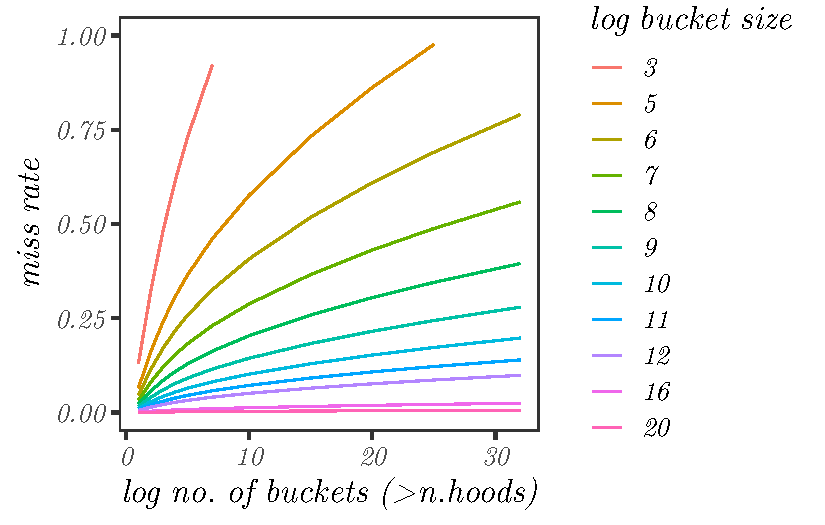
\includegraphics{postage_batch_utilization_figs/fig-mean-1.pdf}

}

}

\subcaption{\label{fig-mean-1}Miss rate against the number of buckets}
\end{minipage}%
%
\begin{minipage}[t]{0.50\linewidth}

{\centering 

\raisebox{-\height}{

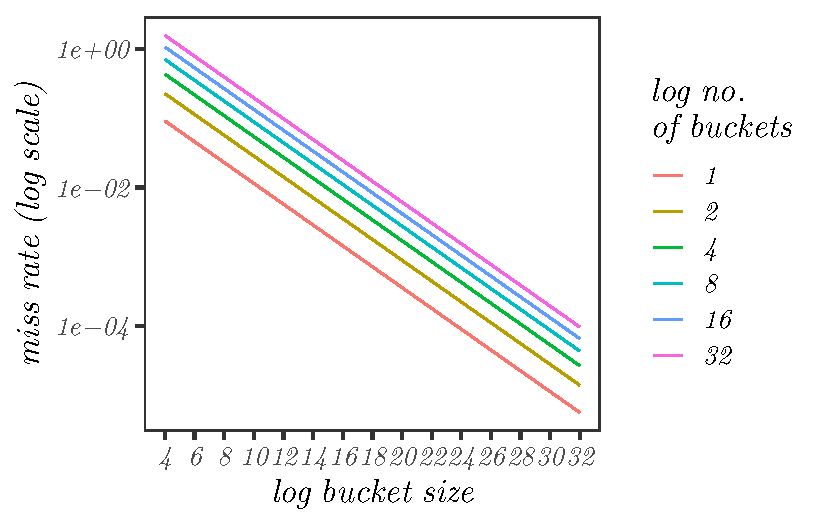
\includegraphics{postage_batch_utilization_figs/fig-mean-2.pdf}

}

}

\subcaption{\label{fig-mean-2}Miss rate against bucket size}
\end{minipage}%

\caption{\label{fig-mean}Expected miss rate, for various parameters.}

\end{figure}

We now investigate the relative standard deviation of the distribution
for various values of $k$ and $n$.

\begin{figure}

\begin{minipage}[t]{0.50\linewidth}

{\centering 

\raisebox{-\height}{

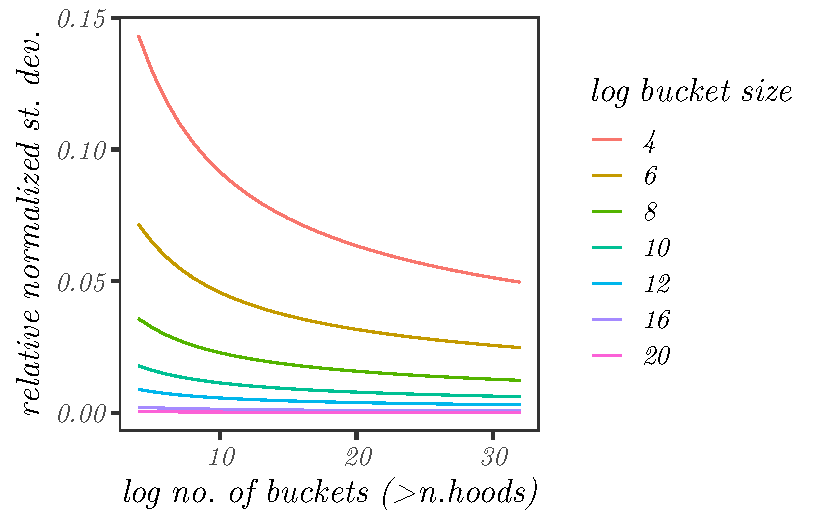
\includegraphics{postage_batch_utilization_figs/fig-sd-1.pdf}

}

}

\subcaption{\label{fig-sd-1}Relative standard deviation against the
number of buckets}
\end{minipage}%
%
\begin{minipage}[t]{0.50\linewidth}

{\centering 

\raisebox{-\height}{

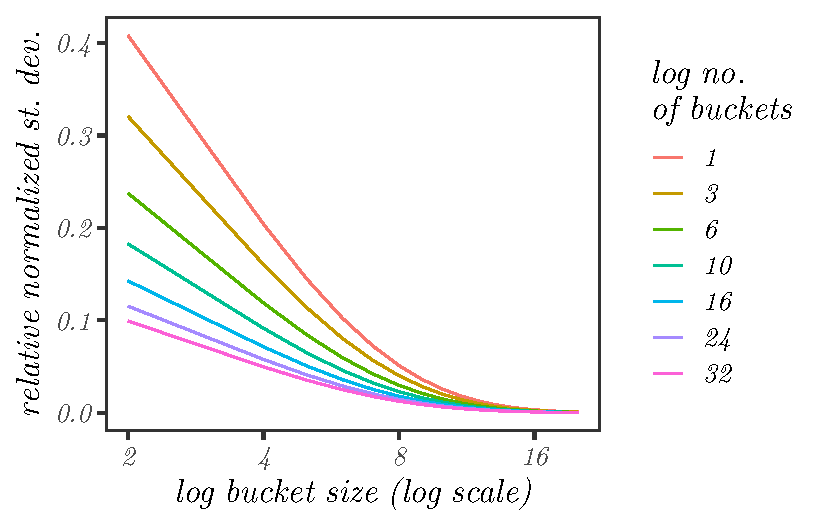
\includegraphics{postage_batch_utilization_figs/fig-sd-2.pdf}

}

}

\subcaption{\label{fig-sd-2}Relative standard deviation against bucket
size}
\end{minipage}%

\caption{\label{fig-sd}Normalized standard deviation of utilization
rate, for various parameters.}

\end{figure}

It is instructive to see that there is not much variance whenever $k$
and $n$ are large. Nevertheless, for the sake of correctness, we check
the quantile function of our extreme value distribution.

\begin{figure}

\begin{minipage}[t]{0.50\linewidth}

{\centering 

\raisebox{-\height}{

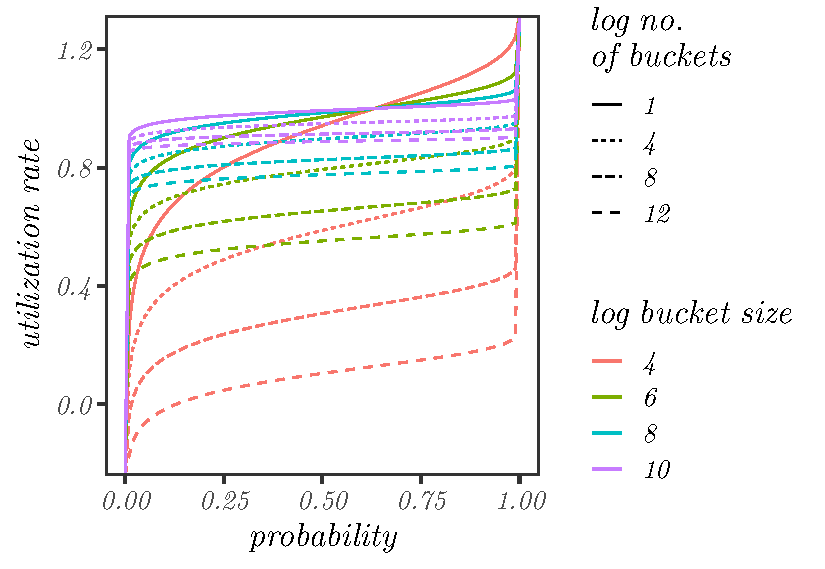
\includegraphics{postage_batch_utilization_figs/fig-qua-1.pdf}

}

}

\subcaption{\label{fig-qua-1}The quantile function of the utilization
rate for various parameters}
\end{minipage}%
%
\begin{minipage}[t]{0.50\linewidth}

{\centering 

\raisebox{-\height}{

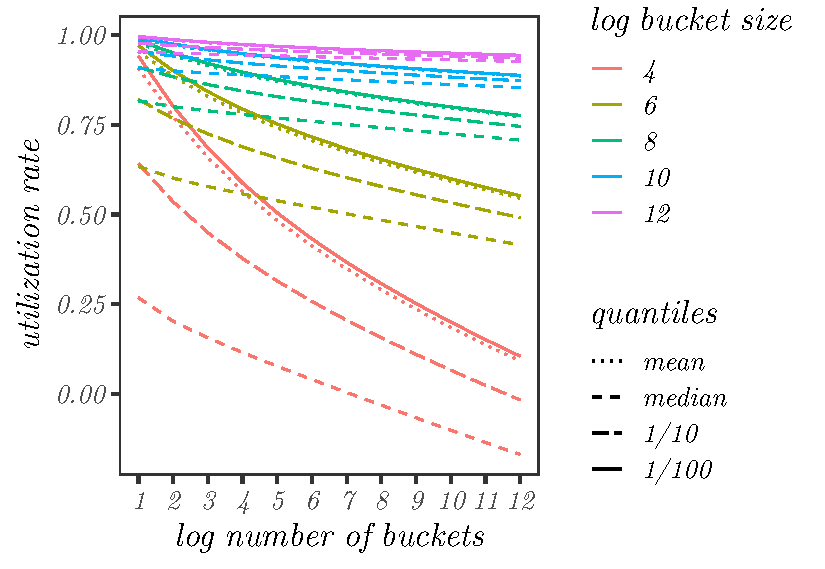
\includegraphics{postage_batch_utilization_figs/fig-qua-2.pdf}

}

}

\subcaption{\label{fig-qua-2}Mean, median, 10\%, and 1\% percentiles of
utilization against number of buckets}
\end{minipage}%

\caption{\label{fig-qua}Quantiles of the utilization function, for
various parameters.}

\end{figure}

\begin{figure}

\begin{minipage}[t]{0.50\linewidth}

{\centering 

\raisebox{-\height}{

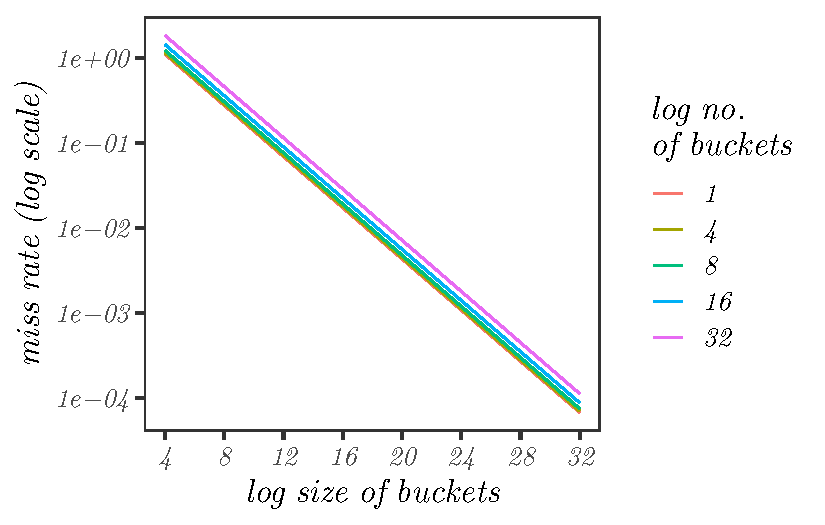
\includegraphics{postage_batch_utilization_figs/fig-q-1.pdf}

}

}

\subcaption{\label{fig-q-1}One-in-a-thousand quantile for miss rate
against bucket size}
\end{minipage}%
%
\begin{minipage}[t]{0.50\linewidth}

{\centering 

\raisebox{-\height}{

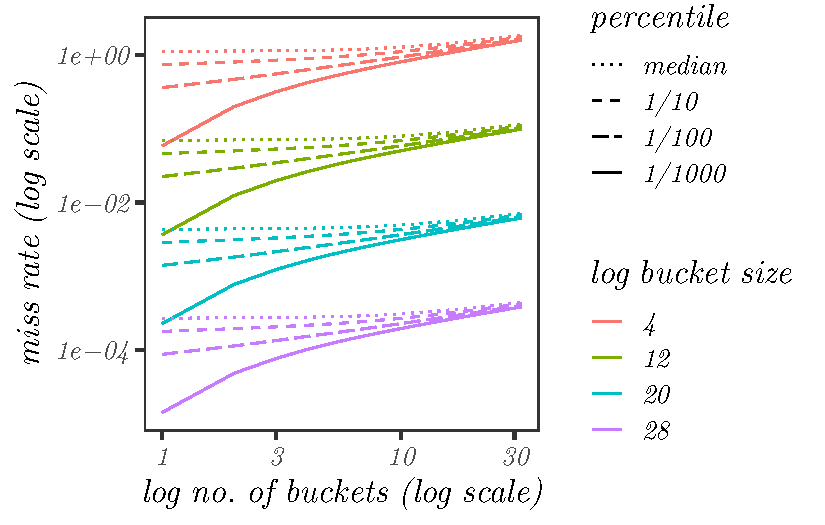
\includegraphics{postage_batch_utilization_figs/fig-q-2.pdf}

}

}

\subcaption{\label{fig-q-2}Miss rate in terms of percentiles, against
number of buckets}
\end{minipage}%

\caption{\label{fig-q}Quantiles of the miss rate for various
parameters.}

\end{figure}

As is clear from the diagram, bucket depth is the major determinant of
the utilization rate. As long as bucket depth is around 8 or greater,
the dependence of the utilization rate on $n$ is milder and milder,
and at $2^{16}$, it is virtually a flat line at $100\%$.

Eventually, we aim to use the information on utilization rates to
protect the user from being surprised at the effective utilization of
their postage batch. To this end, we apply the volume calibration using
a reasonable worst-case scenario, i.e., define the effective utilization
rate as the one-in-a-thousand low-tail quantile of the utilization rate.
To obtain the ``effective'' volumes, we simply multiply the theoretical
purchased volume (given by $2^d$ where $d$ is the batch depth) by
the effective utilization rate.

Finally, we provide these volume calibrations for $2^{12}$ and
$2^{16}$ buckets and log bucket sizes ranging from $4$ to $25$.
Above this bucket size the required quantile already shows a miss rate
below $0.1\%$. That is, there is only a one-in-a-thousand chance that
the difference between the effectively utilized volume and the
theoretically purchased one exceeds one tenth of a percent which we
consider insignificant enough to justify no calibration on the
theoretical volume.

\begin{longtable}[]{@{}
  >{\raggedleft\arraybackslash}p{(\columnwidth - 8\tabcolsep) * \real{0.2941}}
  >{\raggedleft\arraybackslash}p{(\columnwidth - 8\tabcolsep) * \real{0.2500}}
  >{\raggedright\arraybackslash}p{(\columnwidth - 8\tabcolsep) * \real{0.1765}}
  >{\raggedright\arraybackslash}p{(\columnwidth - 8\tabcolsep) * \real{0.1324}}
  >{\raggedright\arraybackslash}p{(\columnwidth - 8\tabcolsep) * \real{0.1471}}@{}}
\toprule()
\begin{minipage}[b]{\linewidth}\raggedleft
log2 no. of buckets
\end{minipage} & \begin{minipage}[b]{\linewidth}\raggedleft
log2 bucket size
\end{minipage} & \begin{minipage}[b]{\linewidth}\raggedright
utilization
\end{minipage} & \begin{minipage}[b]{\linewidth}\raggedright
volume
\end{minipage} & \begin{minipage}[b]{\linewidth}\raggedright
effective
\end{minipage} \\
\midrule()
\endhead
12 & 4 & 0.00000 & 64.00 K & 0.00 B \\
12 & 5 & 0.06747 & 128.00 K & 8.64 K \\
12 & 6 & 0.34060 & 256.00 K & 87.19 K \\
12 & 7 & 0.53374 & 512.00 K & 273.27 K \\
12 & 8 & 0.67030 & 1.00 M & 686.39 K \\
12 & 9 & 0.76687 & 2.00 M & 1.53 M \\
12 & 10 & 0.83515 & 4.00 M & 3.34 M \\
12 & 11 & 0.88343 & 8.00 M & 7.07 M \\
12 & 12 & 0.91758 & 16.00 M & 14.68 M \\
12 & 13 & 0.94172 & 32.00 M & 30.13 M \\
12 & 14 & 0.95879 & 64.00 M & 61.36 M \\
12 & 15 & 0.97086 & 128.00 M & 124.27 M \\
12 & 16 & 0.97939 & 256.00 M & 250.72 M \\
12 & 17 & 0.98543 & 512.00 M & 504.54 M \\
12 & 18 & 0.98970 & 1.00 G & 1013.45 M \\
12 & 19 & 0.99271 & 2.00 G & 1.99 G \\
12 & 20 & 0.99485 & 4.00 G & 3.98 G \\
12 & 21 & 0.99636 & 8.00 G & 7.97 G \\
12 & 22 & 0.99742 & 16.00 G & 15.96 G \\
12 & 23 & 0.99818 & 32.00 G & 31.94 G \\
12 & 24 & 0.99871 & 64.00 G & 63.92 G \\
12 & 25 & 0.99909 & 128.00 G & 127.88 G \\
16 & 4 & 0.00000 & 1.00 M & 0.00 B \\
16 & 5 & 0.00000 & 2.00 M & 0.00 B \\
16 & 6 & 0.28669 & 4.00 M & 1.15 M \\
16 & 7 & 0.49561 & 8.00 M & 3.96 M \\
16 & 8 & 0.64334 & 16.00 M & 10.29 M \\
16 & 9 & 0.74781 & 32.00 M & 23.93 M \\
16 & 10 & 0.82167 & 64.00 M & 52.59 M \\
16 & 11 & 0.87390 & 128.00 M & 111.86 M \\
16 & 12 & 0.91084 & 256.00 M & 233.17 M \\
16 & 13 & 0.93695 & 512.00 M & 479.72 M \\
16 & 14 & 0.95542 & 1.00 G & 978.35 M \\
16 & 15 & 0.96848 & 2.00 G & 1.94 G \\
16 & 16 & 0.97771 & 4.00 G & 3.91 G \\
16 & 17 & 0.98424 & 8.00 G & 7.87 G \\
16 & 18 & 0.98885 & 16.00 G & 15.82 G \\
16 & 19 & 0.99212 & 32.00 G & 31.75 G \\
16 & 20 & 0.99443 & 64.00 G & 63.64 G \\
16 & 21 & 0.99606 & 128.00 G & 127.50 G \\
16 & 22 & 0.99721 & 256.00 G & 255.29 G \\
16 & 23 & 0.99803 & 512.00 G & 510.99 G \\
16 & 24 & 0.99861 & 1.00 T & 1022.57 G \\
16 & 25 & 0.99901 & 2.00 T & 2.00 T \\
\bottomrule()
\end{longtable}



\end{document}
